\documentclass[12pt,twoside]{article}
%%%%%%%%%%%%%%%%%%%%%%%%%%%%%%%%%%%%%%%%%%%%%%%%%%%%%%%%%%%%%
% Meta informations:
\newcommand{\trauthor}{Amy Bryce}
\newcommand{\trtype}{Seminar Paper} %{Seminararbeit} %{Proseminararbeit}
\newcommand{\trcourse}{Bio-Inspired Artificial Intelligence}
\newcommand{\trtitle}{AudioNet: Transfer Learning with a Simplified Version of SoundNet}
\newcommand{\trmatrikelnummer}{7014841}
\newcommand{\tremail}{7bryce@informatik.uni-hamburg.de}
\newcommand{\trarbeitsbereich}{Knowledge Technology, WTM}
\newcommand{\trdate}{31.01.2018}

%%%%%%%%%%%%%%%%%%%%%%%%%%%%%%%%%%%%%%%%%%%%%%%%%%%%%%%%%%%%%
% Languages:

% Falls die Ausarbeitung in Deutsch erfolgt:
% \usepackage[german]{babel}
% \usepackage[T1]{fontenc}
% \usepackage[latin1]{inputenc}
% \usepackage[latin9]{inputenc}
% \selectlanguage{german}

% If the thesis is written in English:
\usepackage[english]{babel}
\selectlanguage{english}

%%%%%%%%%%%%%%%%%%%%%%%%%%%%%%%%%%%%%%%%%%%%%%%%%%%%%%%%%%%%%
% Bind packages:
\usepackage{acronym}                    % Acronyms
\usepackage{algorithmic}                % Algorithms and Pseudocode
\usepackage{algorithm}                  % Algorithms and Pseudocode
\usepackage{amsfonts}                   % AMS Math Packet (Fonts)
\usepackage{amsmath}                    % AMS Math Packet
\usepackage{amssymb}                    % Additional mathematical symbols
\usepackage{amsthm}
\usepackage{booktabs}                   % Nicer tables
%\usepackage[font=small,labelfont=bf]{caption} % Numbered captions for figures
\usepackage{color}                      % Enables defining of colors via \definecolor
\definecolor{uhhRed}{RGB}{254,0,0}      % Official Uni Hamburg Red
\definecolor{uhhGrey}{RGB}{122,122,120} % Official Uni Hamburg Grey
\usepackage{fancybox}                   % Gleichungen einrahmen
\usepackage{fancyhdr}                    % Packet for nicer headers
%\usepackage{fancyheadings}             % Nicer numbering of headlines
\usepackage{fancyvrb}                   % fancybox verbatim
\usepackage{float}                      % so that we can use {H} to position figures in text

%\usepackage[outer=3.35cm]{geometry}     % Type area (size, margins...) !!!Release version
%\usepackage[outer=2.5cm]{geometry}     % Type area (size, margins...) !!!Print version
%\usepackage{geometry}                   % Type area (size, margins...) !!!Proofread version
\usepackage[outer=3.15cm]{geometry}     % Type area (size, margins...) !!!Draft version
\geometry{a4paper,body={5.8in,9in}}

\usepackage{graphicx}                   % Inclusion of graphics
%\usepackage{latexsym}                  % Special symbols
\usepackage{longtable}                  % Allow tables over several parges
\usepackage{listings}                   % Nicer source code listings
\usepackage{multicol}                    % Content of a table over several columns
\usepackage{multirow}                    % Content of a table over several rows
\usepackage[section]{placeins}
\usepackage{rotating}                    % Alows to rotate text and objects
\usepackage{subcaption}                 % subcaption
% \usepackage[hang]{subfigure}            % Allows to use multiple (partial) figures in a fig
%\usepackage[font=footnotesize,labelfont=rm]{subfig}  % Pictures in a floating environment
\usepackage{tabularx}                    % Tables with fixed width but variable rows
\usepackage{url,xspace,boxedminipage}   % Accurate display of URLs

%%%%%%%%%%%%%%%%%%%%%%%%%%%%%%%%%%%%%%%%%%%%%%%%%%%%%%%%%%%%%
% Configurationen:

\hyphenation{whe-ther}                   % Manually use: "\-" in a word: Staats\-ver\-trag

%\lstloadlanguages{C}                   % Set the default language for listings
\DeclareGraphicsExtensions{.pdf,.svg,.jpg,.png,.eps} % first try pdf, then eps, png and jpg
\graphicspath{{./figures/}}             % Path to a folder where all pictures are located
\pagestyle{fancy}                       % Use nicer header and footer

% Redefine the environments for floating objects:
\setcounter{topnumber}{3}
\setcounter{bottomnumber}{2}
\setcounter{totalnumber}{4}
\renewcommand{\topfraction}{0.9}         %Standard: 0.7
\renewcommand{\bottomfraction}{0.5}      %Standard: 0.3
\renewcommand{\textfraction}{0.1}        %Standard: 0.2
\renewcommand{\floatpagefraction}{0.8}   %Standard: 0.5

% Tables with a nicer padding:
\renewcommand{\arraystretch}{1.2}

%%%%%%%%%%%%%%%%%%%%%%%%%%%%
% Additional 'theorem' and 'definition' blocks:
\theoremstyle{plain}
\newtheorem{theorem}{Theorem}[section]
%\newtheorem{theorem}{Satz}[section]    % Wenn in Deutsch geschrieben wird.
\newtheorem{axiom}{Axiom}[section]
%\newtheorem{axiom}{Fakt}[chapter]      % Wenn in Deutsch geschrieben wird.
%Usage:%\begin{axiom}[optional description]%Main part%\end{fakt}

\theoremstyle{definition}
\newtheorem{definition}{Definition}[section]

%Additional types of axioms:
\newtheorem{lemma}[axiom]{Lemma}
\newtheorem{observation}[axiom]{Observation}

%Additional types of definitions:
\theoremstyle{remark}
%\newtheorem{remark}[definition]{Bemerkung} % Wenn in Deutsch geschrieben wird.
\newtheorem{remark}[definition]{Remark}

%%%%%%%%%%%%%%%%%%%%%%%%%%%%
% Provides TODOs within the margin:
\newcommand{\TODO}[1]{\marginpar{\emph{\small{{\bf TODO: } #1}}}}

%%%%%%%%%%%%%%%%%%%%%%%%%%%%
% Abbreviations and mathematical symbols
\newcommand{\modd}{\text{ mod }}
\newcommand{\RS}{\mathbb{R}}
\newcommand{\NS}{\mathbb{N}}
\newcommand{\ZS}{\mathbb{Z}}
\newcommand{\dnormal}{\mathit{N}}
\newcommand{\duniform}{\mathit{U}}

\newcommand{\erdos}{Erd\H{o}s}
\newcommand{\renyi}{-R\'{e}nyi}
%%%%%%%%%%%%%%%%%%%%%%%%%%%%%%%%%%%%%%%%%%%%%%%%%%%%%%%%%%%%%
% Document:
\begin{document}
\renewcommand{\headheight}{14.5pt}

\fancyhead{}
\fancyhead[LE]{ \slshape \trauthor}
\fancyhead[LO]{}
\fancyhead[RE]{}
\fancyhead[RO]{ \slshape \trtitle}

%%%%%%%%%%%%%%%%%%%%%%%%%%%%
% Cover Header:
\begin{titlepage}
  \begin{flushleft}
    Universit\"at Hamburg\\
    Department Informatik\\
    \trarbeitsbereich\\
  \end{flushleft}
  \vspace{3.5cm}
  \begin{center}
    \huge \trtitle\\
  \end{center}
  \vspace{3.5cm}
  \begin{center}
    \normalsize\trtype\\
    [0.2cm]
    \Large\trcourse\\
    [1.5cm]
    \Large \trauthor\\
    [0.2cm]
    \normalsize Matr.Nr. \trmatrikelnummer\\
    [0.2cm]
    \normalsize\tremail\\
    [1.5cm]
    \Large \trdate
  \end{center}
  \vfill
\end{titlepage}

  %backsite of cover sheet is empty!
\thispagestyle{empty}
\hspace{1cm}
\newpage


%%%%%%%%%%%%%%%%%%%%%%%%%%%
%% Abstract
%%%%%%%%%%%%%%%%%%%%%%%%%%%
\section*{Abstract}
Audio event detection is comparatively less advanced than speech and image recognition.
A major reason for this is the lack of labeled natural sound datasets for audio classifiers to train on, whereas speech and image classifiers have massive amounts of data available to them.
Generally, the more data we have to work with, the more accurate we can become at classifying natural sounds.
SoundNet, a deep sound network developed by researchers at MIT~\cite{Aytar:Yusuf:16}, contributes to the solution by generating a dataset of labeled natural sound using a training process called transfer learning~\cite{Yosinski:2014}.
SoundNet does this by leveraging the natural correlation between sound and images in videos to train an audio classifier using the outputs from an established pretrained image classifier.
This effectively transfers the knowledge from the image classifier to the audio classifier.
In this paper, we introduce AudioNet, our simplified implementation of SoundNet.
We successfully train AudioNet to classify sounds from unlabeled videos using the transfer learning process and discuss the details of how data flows through our network.

% Lists:
\setcounter{tocdepth}{2}           % depth of the table of contents (for Seminars 2 is recommented)
\tableofcontents
\pagenumbering{arabic}
\clearpage

%%%%%%%%%%%%%%%%%%%%%%%%%%%%
% Content:

% the actual content, usually separated over a number of sections
% each section is assigned a label, in order to be able to put a
% crossreference to it


%%%%%%%%%%%%%%%%%%%%%%%%%%%
%%  Introduction
%%%%%%%%%%%%%%%%%%%%%%%%%%%
\section{Introduction}
\label{sec:introduction}
With the increase of audio processing technology, there is a need for smarter and more accurate audio event detection.
Over the last decade, there have been significant improvements in speech recognition (ASR) and Music Information Retrieval (MIR)~\cite{Stowell:2015}, but detecting and classifying natural sound is comparatively further behind.
One reason for this is the scarcity of large datasets of labeled natural sound~\cite{Aytar:Yusuf:16}.
SoundNet, a deep sound network~\cite{Aytar:Yusuf:16}, attempts to address this problem by leveraging an established image classifier to train their network through a process called transfer learning~\cite{Yosinski:2014}.
The result is “a large-scale and semantically rich [dataset] for natural sound”~\cite{Aytar:Yusuf:16}.
We believe that transfer learning is at the crux of this contribution.
However, given SoundNet’s deep nature, it is difficult to explain it’s full training process end to end.

For the purpose of this paper, our intention was not to build a robust solution to classify sound.
Instead, our goal was to design a simplified version of SoundNet, called AudioNet, to make it easier to explain training a neural network and how transfer learning works in detail.
In our implementation, transfer learning is accomplished by teaching AudioNet to classify sounds using the output of a pretrained image classifier inferring on associated images.
To do this, we selected ten videos representing ten different categories, split them into an image track and an audio track, and then fed them through our classifiers.
Our goal was for the output of the pretrained image classifier to help guide AudioNet into understanding how to classify the associated audio that it was given.

Normally, we’d want to train our classifier with as many sounds as possible to prevent overfitting.
However, for the purpose of scaling down this project to focus on transfer learning, overfitting was a necessary side effect.
As a result, it was expected that AudioNet would only be able to accurately classify sounds that it was trained on.
We will address this in Section~\ref{sec:evaluation}, and discuss how, with enough iterations, AudioNet was able to successfully classify these sounds.

The rest of this paper is structured as follows.
In Section~\ref{sec:background}, we briefly define some concepts and key terms that we’ll be referencing in this paper.
In Section~\ref{sec:architecture}, we go over the architecture of AudioNet on a high level before we dive deeper into how it was implemented in Section~\ref{sec:implementation}.
In Section~\ref{sec:evaluation}, we discuss how we fine-tuned aspects of our implementation to get the results we’d expect and the issues that we encountered as a result.
Finally, in Section~\ref{sec:conclusion}, we conclude with summarizing this paper.


%%%%%%%%%%%%%%%%%%%%%%%%%%%
%%  Background
%%%%%%%%%%%%%%%%%%%%%%%%%%%
\section{Background}
\label{sec:background}
In order to understand how AudioNet is structured and operates, we need to define a few key concepts first.
It will become clear throughout the rest of this paper how these concepts are used.

\bigskip
\noindent
\textbf{Classifier:}
For the purpose of this paper, a classifier is defined as a neural network that takes an input and classifies it into a set of categorized outputs.
Examples of this include vgg16~\cite{Simonyan:2014}, SoundNet, and even AudioNet.

\bigskip
\noindent
\textbf{Convolutional Layer:}
A layer in a neural network that extracts features from an input by examining sections of the input, rather than considering the entire input at once.
The result is being able to detect a particular feature no matter where it exists in a given input.
In AudioNet, we use this layer to extract features from an audio signal.

\bigskip
\noindent
\textbf{Pooling Layer:}
In this paper we use two types of pooling layers: a max pooling layer and an average pooling layer.
A max pooling layer takes the highest values detected in a feature and pools them together.
An average pooling layer then takes these pooled values and averages them to produce a single value representing the feature.

\bigskip
\noindent
\textbf{Dense Linear Layer:}
Also known as a fully connected layer, a dense linear layer is the classic hidden layer of a neural network.
In contrast to a convolutional layer, a dense linear layer is designed to detect features over the entire input.
In AudioNet, we use this as our final layer to classify the original input based on the features extracted from the convolutional layer and the pooling layers.

\bigskip
\noindent
\textbf{Loss Function:}
Also known as a cost function, the loss function is used to compute the error in a network being trained against a target value.
There are many different algorithms available to compute the error.
The loss function that SoundNet and AudioNet use is KL-Divergence~\cite{kullback:68a}.
We compute the KL-Divergence between our output from AudioNet and the output of vgg16 as our target.

\bigskip
\noindent
\textbf{Backpropagation:}
After feeding input through a neural network and computing a loss function, the network needs to be updated to increase its accuracy.
Backpropagation is a technique used to walk back through the network under training and compute the gradients on all the nodes at each layer~\cite{ChauvinRumelhart95}.
An optimizer is then used to update the weights on those nodes using the gradients that were just calculated.
The optimizer we chose to use in AudioNet is Stochastic Gradient Descent (SGD)~\cite{Bottou:2010}.

\bigskip
\noindent
\textbf{Overfitting:}
Overfitting is something that happens to a classifier during the training process when it is shown the same inputs too often.
This forces it to memorize patterns in those specific inputs, rather than learning to recognize common patterns that would allow it to classify new inputs correctly.
As mentioned previously, we purposefully overfit AudioNet to only accurately classify sounds from the videos it was trained on.


%%%%%%%%%%%%%%%%%%%%%%%%%%%
%%  Architecture
%%%%%%%%%%%%%%%%%%%%%%%%%%%
\section{Architecture}
\label{sec:architecture}
This section describes our architecture for AudioNet.
Its purpose is to demonstrate transfer learning by classifying sounds using the output of a pretrained image classifier inferring on associated images.
Figure~\ref{fig:audionet_architecture} shows a more detailed representation of this process.

\begin{figure}[H]
   \centerline{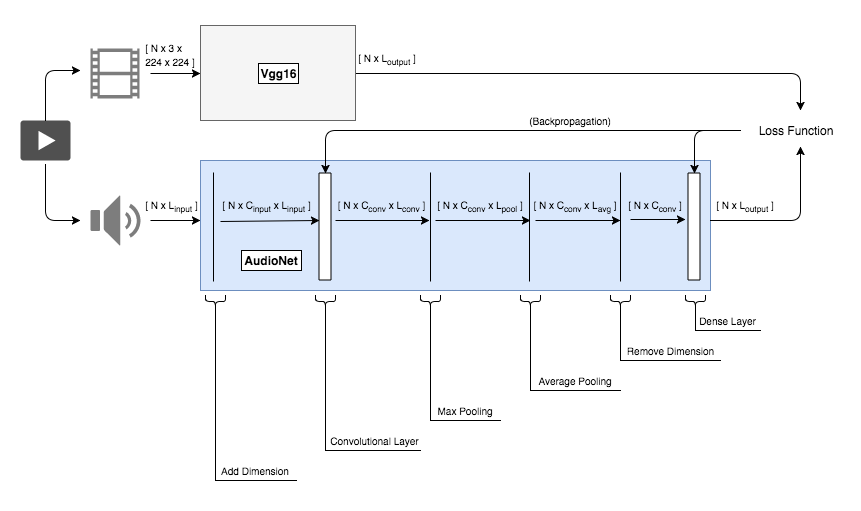
\includegraphics[width=\textwidth]{audionet_architecture.png}}
   {\caption{\footnotesize An overview of the AudioNet architecture showing the training process.}
     \label{fig:audionet_architecture}}
\end{figure}

We begin by separating unlabeled videos into two tracks, an audio track and an image track.
We then feed the audio track through AudioNet, and the image track through a well known pretrained image classifier called vgg16~\cite{Simonyan:2014}.
The outputs of both classifiers are probability distributions representing the likelihood that the inputs fall into one of a thousand different categories.
These categories are defined by the ImageNet database of labeled images~\cite{Deng:2009}.
The goal is to train AudioNet to produce a probability distribution for an audio segment that mimics vgg16’s probability distribution with a corresponding image segment.
This is accomplished by computing their differences in a loss function, calculating gradients, backpropagating the gradients through AudioNet, and updating its weights so that it will become more accurate during the next iteration of training.

AudioNet itself is a neural network consisting of four distinct layers: a convolutional layer, a max pooling layer, an average pooling layer, and a dense linear layer.
The convolutional layer extracts features from the input, the pooling layers highlight the strongest features, and the dense linear layer translates these features into a probability distribution representing the likelihood that those features match a particular category.
The convolutional layer and the dense linear layer are the only layers that have nodes whose weights are updated after backpropagation.

As seen in Figure~\ref{fig:audionet_architecture}, the dimensionality of the input changes as it flows through each layer.
These changes are dependent on how the properties of each layer are configured.
We’ll go into the details on how this was done in the following section.


%%%%%%%%%%%%%%%%%%%%%%%%%%%
%%  Implementation
%%%%%%%%%%%%%%%%%%%%%%%%%%%
\section{Implementation}
\label{sec:implementation}
We implemented the architecture of AudioNet using \texttt{pytorch}~\cite{pytorch}.
We created four \texttt{python} modules: \texttt{frames.py}, \texttt{train.py}, \texttt{audionet.py}, and \texttt{infer.py}.
Figure~\ref{fig:module_diagram} shows the interaction of these modules for training AudioNet and using it for inference.

\begin{figure}[H]
   \centerline{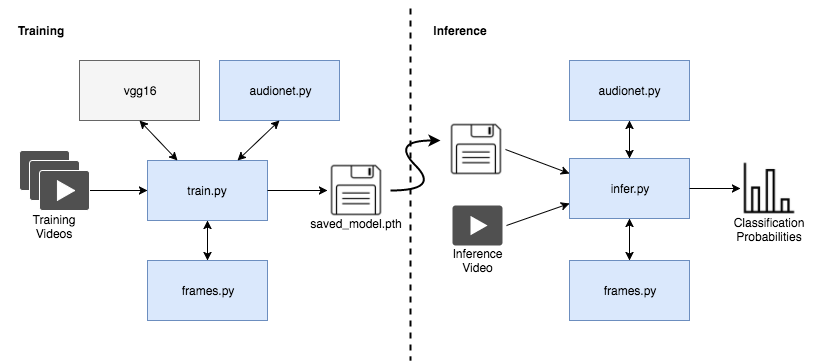
\includegraphics[width=\textwidth]{module_diagram.png}}
   {\caption{\footnotesize An overview of the interaction between our AudioNet python modules.}
     \label{fig:module_diagram}}
\end{figure}

\bigskip
\noindent
\textbf{\texttt{frames.py:}}
This module is responsible for taking unlabeled video files and separating them into an audio track and an image track.
Within this module, we define a function called \texttt{get()} that accepts three parameters:
a video file, a video sample period, and an audio sampling rate.
We set a default video sample period of $40ms$ and an audio sampling rate of $16kHz$.

\noindent
\begin{center}
\texttt{get(video\_file, sample\_period\_msec = 40, audio\_sample\_rate = 16000)}
\end{center}

\noindent
Within this function, we use \texttt{moviepy} to first read in the video file and break it into frames, where the length of each frame matches the video sample period.
Then for each frame, we extract the image in the middle of that frame and subsample the audio across the entire frame at the audio sampling rate.
Once we’ve done this for every frame, we return a list of all the extracted images along with their associated audio samples.
A full implementation of this module can be found in Appendix~\ref{subsec:frames.py}.

\bigskip
\noindent
\textbf{\texttt{train.py:}}
This module is responsible for training AudioNet to classify sounds into the thousand categories defined by ImageNet.
It runs as a script that accepts two arguments:
the path specifying where to save the trained model, and a list of videos to train on.

\noindent
\begin{center}
\texttt{train.py -o <saved\_model\_path> <video\_file>...}
\end{center}

\noindent
We begin by reading in the video files, iterating over them, and extracting their image tracks and audio tracks.
For every set of tracks we extract, we format them for processing, pair the corresponding frames from each track, and add them to a list of paired frames.
Once this has completed, we shuffle the entire list to randomize the order of paired frames that will be passed through the training process.
The pseudo code below summarizes how this is done:

{\setlength{\fboxsep}{10pt}
\begin{Verbatim}[frame=leftline, numbers=left, xleftmargin=5mm]
paired_frames = []
foreach video_file in video_files:
    image_track, audio_track = frames.get(video_file)
    image_track = format_images(image_track)
    audio_track = format_audio(audio_track)
    for image_frame, audio_frame in image_track, audio_track:
        paired_frames.append((image_frame, audio_frame))

paired_frames = shuffle(paired_frames)
\end{Verbatim}
}

AudioNet and vgg16 expect their inputs to be formatted in a particular way.
For vgg16, we need to apply three different transformations to the raw image frames:
(1) convert each image frame into an RGB image using the \texttt{python} \texttt{PIL} image library~\cite{pil},
(2) resize each image frame to $224 \times 224$ pixels, and
(3) normalize each image frame to have a specific mean and standard deviation~\cite{vgg}.
AudioNet simply accepts raw audio samples as input.
However, before we feed these formatted inputs into AudioNet and vgg16, we need to convert them into \texttt{pytorch.Tensor} types and wrap them in a \texttt{pytorch.autograd.Variable}.
This last step is important because this allows us to leverage \texttt{pytorch}’s built-in ability to compute gradients and backpropagate them through AudioNet (we will discuss this in more detail below).

We then feed each frame in our formatted image track through vgg16 to produce an output probability distribution.
Likewise, we feed each frame in our formatted audio track through AudioNet to produce its own output probability distribution.
We take these outputs and compute their KL-Divergence as our loss function.
As we feed more and more input frames through our classifiers, the goal is to minimize this KL-Divergence over time.
To accomplish this, we use \texttt{pytorch}’s autograd library to compute the gradient on the loss function and backpropagate this computation through AudioNet.
We then apply Stochastic Gradient Descent (SGD)~\cite{Bottou:2010} to update the weights in AudioNet’s convolutional and dense linear layers using these computed gradients.

In general, using a small learning rate when applying SGD helps prevent overfitting.
Therefore, we used a very small learning rate of $1e-4$.
However, with the intent of implementing a simplified audio classifier to demonstrate transfer learning, we purposely designed our training loop to overfit on the specific videos we train it on.
This ensures that AudioNet is able to accurately classify sounds from the videos it trains on, but \textit{cannot} guarantee it will be able to classify sounds from unfamiliar videos.

In order to increase AudioNet’s accuracy when categorizing sounds, we train it on the full set of paired frames multiple times.
Each pass through the full set of paired frames constitutes one epoch.
While iterating over multiple epochs increases training time, processing the paired frames in batches can help decrease training time.
The number of epochs and batch size can be tuned based on how long you are willing wait and what hardware you have available.
We discuss this further in Section~\ref{sec:evaluation}.

Once we’ve processed every batch, over a number of epochs, we save the trained model to an output file.
The pseudo code for the aforementioned process is pictured below.
A full implementation of this module can be found in Appendix~\ref{subsec:train.py}.

{\setlength{\fboxsep}{10pt}
\begin{Verbatim}[frame=leftline, numbers=left, xleftmargin=5mm]
optimizer = sgd(learning_rate)

for epoch in range(num_epochs):
    for batch in iterate(paired_frames, batch_size):
        image_frames = batch[0]
        audio_frames = batch[1]

        vgg_output = vgg16(image_frames)
        audionet_output = audionet(audio_frames)

        loss = kldiv(input = audionet_output, target = vgg_output)
        loss.backward()

        optimizer.step()

audionet.save(“saved_model.pth”)
\end{Verbatim}
}

\bigskip
\noindent
\textbf{\texttt{audionet.py:}}
This module is responsible for implementing the core logic of AudioNet itself.
We define a class called \texttt{audionet} that extends from \texttt{pytorch.nn.Module}.
In the \texttt{init()} function of this class, we create instances of \texttt{pytorch}’s built-in classes for \texttt{Conv1d}, \texttt{MaxPool1d}, \texttt{avg\_pool1d}, and \texttt{Linear} from \texttt{pytorch.nn}.
These classes map to each of the layers visible in Figure~\ref{fig:audionet_architecture}.
We configure each of these layers with the properties shown in Table~\ref{tab:layer_properties}.

\begin{table}[H]
\footnotesize
\centering
\begin{tabular}{ |c|c|c|c|c|c| }
\hline
Layer & Input Dimension & Kernel Size & Padding & Stride & Output Dimension \\
\hline
Convolutional & $N \times 1 \times L_{input}$ & $64$ & $32$ & $2$ & $N \times 16 \times L_{conv}$ \\
Max Pooling & $N \times 16 \times L_{conv}$ & $8$ & $4$ & $1$ & $N \times 16 \times L_{pool}$ \\
Average Pooling & $N \times 16 \times L_{pool}$ & $L_{pool}$ & $-$ & $-$ & $N \times 16 \times 1$ \\
Dense Linear & $N \times 16$ & $1000$ & $-$ & $-$ & $N \times 1000$ \\
\hline
\end{tabular}
{\caption{\footnotesize Each layer in AudioNet has tunable parameters.
          This table shows the values we set for each parameter.}
  \label{tab:layer_properties}}
\end{table}

\noindent
We define \texttt{audionet}'s \texttt{forward()} function to accept an input with dimensionality $N \times L_{input}$ and feed it through each of these layers.
$N$ represents the batch size and $L\_input$ represents the length of an audio frame wrapped in a \texttt{pytorch.autograd.Variable}.
The dimensionality of the input changes as it flows through each layer.
The only constant at each layer is $N$.
Because our convolutional layer expects an input channel to be defined, we use the \texttt{pytorch} \texttt{unsqueeze()} method to add another dimension to the initial input.
Likewise, we need to remove a dimension before passing our averaged input through the dense linear layer by using the \texttt{pytorch} \texttt{squeeze()} method.
The resulting output is a probability distribution with a dimensionality of $N \times 1000$.
A full implementation of this module can be found in Appendix~\ref{subsec:audionet.py}.

\bigskip
\noindent
\textbf{\texttt{infer.py:}}
This module is responsible for taking a pretrained AudioNet model and using it to classify sounds from an unlabeled video.
It runs as a script that accepts three arguments:
the path specifying a saved trained model, a video to infer over, and a video sample period.

\noindent
\begin{center}
\texttt{infer.py <saved\_model\_path> <video\_file> <sample\_period>}
\end{center}

\noindent
We begin by loading the saved trained model into \texttt{audionet}.
We then call \texttt{frames.get()} with the sample period to separate the video into two tracks.
Finally, we pass the audio track through \texttt{audionet} to produce a probability distribution for each processed audio frame and dump the results into an output file.
We ignore the image track altogether.
The pseudo code for this can be seen below.
A full implementation of this module can be found in Appendix~\ref{subsec:infer.py}.

{\setlength{\fboxsep}{10pt}
\begin{Verbatim}[frame=leftline, numbers=left, xleftmargin=5mm]
image_track, audio_track = frames.get(video_file, sample_period)
audionet = audionet.loadModel(saved_model_path)

probabilities = []
for audio_frame in audio_track:
    audionet_output = audionet(audio_frame)
    probabilities.append(audionet_output)

save_file(probabilities)
\end{Verbatim}
}


%%%%%%%%%%%%%%%%%%%%%%%%%%%
%%  Evaluation
%%%%%%%%%%%%%%%%%%%%%%%%%%%
\section{Evaluation}
\label{sec:evaluation}
We trained AudioNet using a set of ten videos from Google’s AudioSet, “a large-scale dataset of manually annotated audio events” collected from $10s$ YouTube video clips~\cite{Gemmeke:Jort:17}.
We chose videos from AudioSet as a way to ensure that we could train AudioNet with images and sounds that correlated with one another.
SoundNet, in contrast, uses a large dataset of unlabeled videos from Flickr~\cite{flickr} to train on, making it a more robust audio classifier.
Table~\ref{tab:videos} lists the video clips that we chose.

% Table of videos
\begin{table}[H]
\scriptsize
\centering
\begin{tabular}{ |l|l|c|c| }
\hline
Video Contents & Youtube URL & Start Time & Length \\
\hline
Rooster (Cock) & \url{https://www.youtube.com/watch?v=67GZuUxV27w&t=30} & $00:30$ & $10s$ \\
Sewing Machine & \url{https://www.youtube.com/watch?v=9PmzQI8ZYpg&t=30} & $00:30$ & $10s$ \\
Fire Truck & \url{https://www.youtube.com/watch?v=_A30xsFBMXA&t=40} & $00:40$ & $10s$ \\
Harmonica & \url{https://www.youtube.com/watch?v=BUGx2e7OgFE&t=30} & $00:30$ & $10s$ \\
Polaroid Camera & \url{https://www.youtube.com/watch?v=eHIlPlNWISg&t=90} & $01:30$ & $10s$ \\
Race Car & \url{https://www.youtube.com/watch?v=eV5JX81GzqA&t=150} & $2:30$ & $10s$ \\
Electric Guitar & \url{https://www.youtube.com/watch?v=-OAyRsvFGgc&t=30} & $00:30$ & $10s$ \\
Tree Frog & \url{https://www.youtube.com/watch?v=rctt0dhCHxs&t=16} & $00:16$ & $9s$ \\
Keyboard & \url{https://www.youtube.com/watch?v=rTh92nlG9io&t=30} & $00:30$ & $10s$ \\
Magpie & \url{https://www.youtube.com/watch?v=-XilaFMUwng&t=50} & $00:50$ & $10s$ \\
\hline
\end{tabular}
{\caption{\footnotesize A list of videos used to train AudioNet.
          These videos were obtained from Google's AudioSet~\cite{Gemmeke:Jort:17}.}
  \label{tab:videos}}
\end{table}

As mentioned in Section~\ref{sec:implementation}, there are a number of parameters that we can tune while training AudioNet.
These are the \textbf{number of epochs}, \textbf{batch size}, \textbf{video sample period}, \textbf{audio sampling rate}, and \textbf{learning rate} (for SGD).
The values we set for these parameters during our training can be seen in Table~\ref{tab:tunable_parameters}.

% Table of tunable parameters
\begin{table}[H]
\footnotesize
\centering
\begin{tabular}{ |l|c| }
\hline
Parameter & Value \\
\hline
Epochs & $5000$ \\
Batch Size & $512$ \\
Video Sample Period & $40ms$ \\
Audio Sampling Rate & $16kHz$ \\
Learning Rate & $1e-4$ \\
\hline
\end{tabular}
{\caption{\footnotesize The five tunable parameters for AudioNet’s training process.}
  \label{tab:tunable_parameters}}
\end{table}

We trained AudioNet on a machine containing four NVIDIA Tesla M60 GPUs with 8GB of RAM each~\cite{nvidia}.
As seen in Table~\ref{tab:tunable_parameters}, we were able to choose a large number of epochs and a large batch size because we had these GPUs available.
We could have used a larger batch size, but we were limited by the amount of memory available on each GPU (between 6.5-7GB of RAM were consumed on each GPU with a batch size of 512).
Even with these GPUs, training with a batch size of 512 over 5000 epochs took about 9 hours to complete.

While training AudioNet, we kept track of the KL-Divergence computed for every frame passing through it.
This included all frames from all videos over all epochs.
Once training was completed, we averaged the KL-Divergence computed across all frames in each video on a per epoch basis.
We then plotted these averages in Figure~\ref{fig:kldivs-plot}.

% KL-Div figures
\begin{figure*}[h!]
    \centering
    \begin{subfigure}[t]{0.5\textwidth}
        \centering
        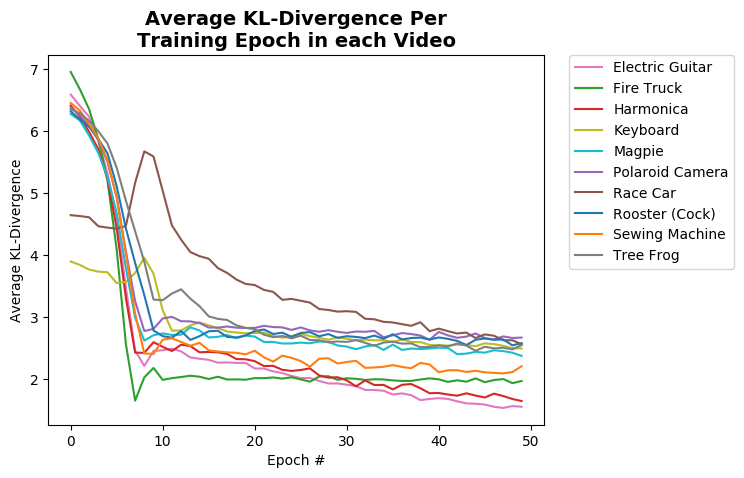
\includegraphics[width=\textwidth]{final_saved_model.pth.stats.json-kldivs-0-50-plot.png}
        {\caption{\footnotesize Epochs $0-50$}
          \label{fig:kldivs-0-50-plot}}
    \end{subfigure}%
    ~
    \begin{subfigure}[t]{0.5\textwidth}
        \centering
        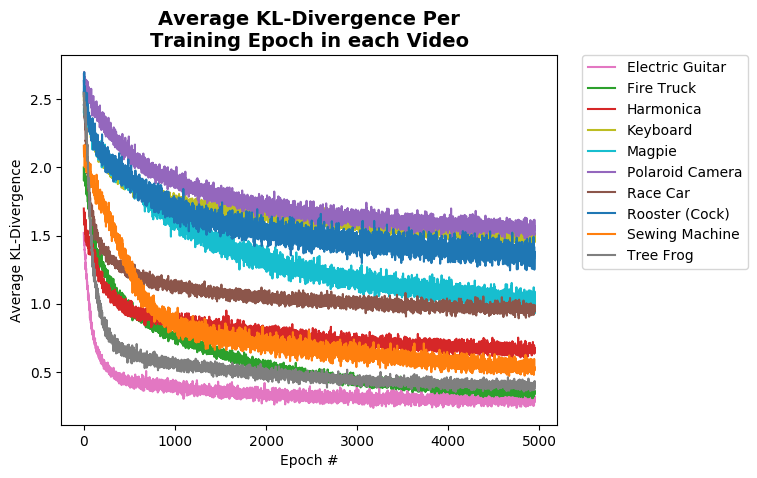
\includegraphics[width=\textwidth]{final_saved_model.pth.stats.json-kldivs-50-5000-plot.png}
        {\caption{\footnotesize Epochs $50-5000$}
          \label{fig:kldivs-50-5000-plot}}
    \end{subfigure}
    {\caption{\footnotesize The KL-Divergence computed between the outputs from AudioNet and vgg16 for all training videos.
              In \ref{fig:kldivs-0-50-plot}, we zoom in on epochs $0-50$ to show the range where the KL-Divergence is most volatile.
              In \ref{fig:kldivs-50-5000-plot}, we show the range $50-5000$ where the KL-Divergence is less volatile and continuously decreases.}
      \label{fig:kldivs-plot}}
\end{figure*}

During the first ten epochs, the KL-Divergence trends down quickly.
By the time we reach 50 epochs, the KL-Divergence for all the videos is between two and three.
And by the time we reach 5000 epochs, the KL-Divergence for all the videos is between one and two.
This downward trend shows that as we train over more epochs, AudioNet’s ability to classify audio begins to more closely mimic the output of the vgg16 image classifier.
Although this looks promising, we want to remind the reader that these trends are a result of overfitting on a small sample of videos.
To reiterate, our goal was not to build a robust audio classifier, but to demonstrate transfer learning between two classifiers.
The results in Figure~\ref{fig:kldivs-plot} demonstrate this process of transfer learning sufficiently.

Once AudioNet was fully trained, we passed each of our ten videos back through it in order to see how well it could classify their associated audio.
In this section, we specifically focus on the results from three specific videos.
Figure~\ref{fig:inf_electric_guitar}, Figure~\ref{fig:inf_polaroid_camera}, and Figure~\ref{fig:inf_keyboard} show the top three most probable sounds that AudioNet is able to classify in the electric guitar, polaroid camera, and computer keyboard videos.
The graphs for the remaining seven videos can be found in Appendix~\ref{sec:additional_figures}.

% Electric Guitar
\begin{figure}[H]
   \centerline{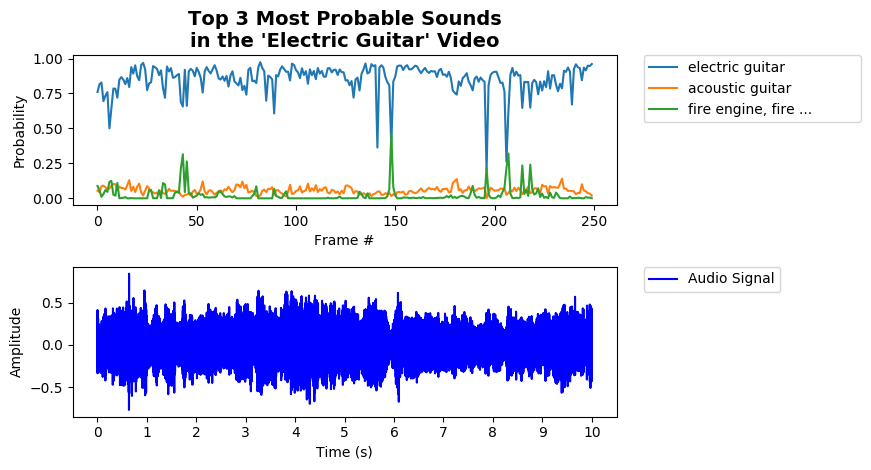
\includegraphics[width=\textwidth]{inf_electric_guitar.png}}
   {\caption{\footnotesize The top graph shows the top three most probable sounds that AudioNet is able to classify from the electric guitar video for each frame.
             The bottom graph shows the raw audio signal from this video over the same time period.}
     \label{fig:inf_electric_guitar}}
\end{figure}

% Polaroid Camera
\begin{figure}[H]
   \centerline{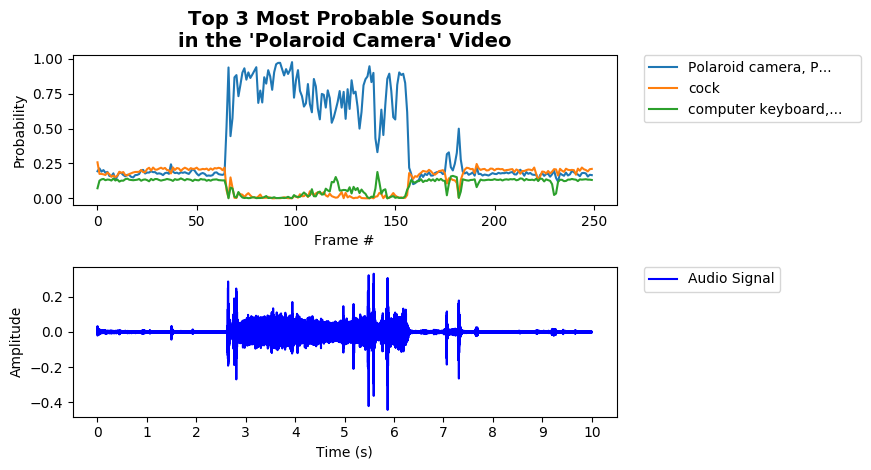
\includegraphics[width=\textwidth]{inf_polaroid_camera.png}}
   {\caption{\footnotesize The top graph shows the top three most probable sounds that AudioNet is able to classify from the polaroid camera video for each frame.
             The bottom graph shows the raw audio signal from this video over the same time period.}
     \label{fig:inf_polaroid_camera}}
\end{figure}

% Computer Keyboard
\begin{figure}[H]
   \centerline{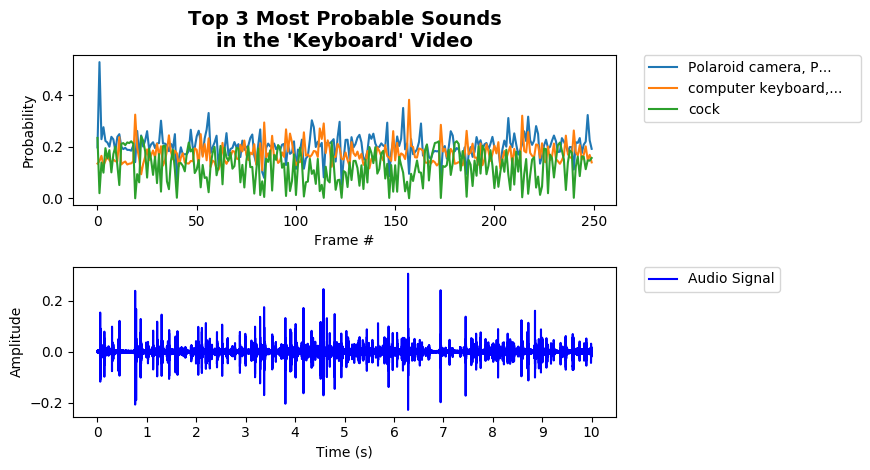
\includegraphics[width=\textwidth]{inf_keyboard.png}}
   {\caption{\footnotesize The top graph shows the top three most probable sounds that AudioNet is able to classify from the computer keyboard video for each frame.
             The bottom graph shows the raw audio signal from this video over the same time period.}
     \label{fig:inf_keyboard}}
\end{figure}

In Figure~\ref{fig:inf_electric_guitar}, we see that AudioNet was very successful at classifying the sounds of an electric guitar.
Likewise, Figure~\ref{fig:inf_polaroid_camera} shows that AudioNet was very successful at classifying the sounds from a polaroid camera.
However, when the audio signal was weak, AudioNet struggled to confidently classify it.
The periods of weak audio signals are often mistaken for a rooster (cock) or a computer keyboard.
A more extreme example of this problem can be seen in Figure~\ref{fig:inf_keyboard}.
This Figure shows the results from the computer keyboard video.
The audio signal from this video is mostly weak, with intermittent bursts of distinctive keyboard sounds.
Over the course of the video, AudioNet misclassified the sounds as a polaroid camera more often than a computer keyboard.

Looking back at Figure~\ref{fig:kldivs-plot}, we can see that the KL-Divergence for the electric guitar video was very low, while the KL-Divergence for the computer keyboard was comparatively much higher.
This is a good indicator as to why Figure~\ref{fig:inf_electric_guitar} and Figure~\ref{fig:inf_keyboard} had such widely varying results.


%%%%%%%%%%%%%%%%%%%%%%%%%%%
%%  Conclusion
%%%%%%%%%%%%%%%%%%%%%%%%%%%
\section{Conclusion}
\label{sec:conclusion}
The primary goal of this paper was to demonstrate transfer learning between two classifiers with a simplified version of SoundNet, called AudioNet.
We presented the overall architecture of AudioNet, followed by details of how it was implemented.
We then evaluated how well our implementation was able to achieve transfer learning.
What we found was that AudioNet was able to classify audio clips during periods where the signal was strong, but struggles with periods where the signal was weak.
Moreover, AudioNet only works well on the specific videos that it was trained on.
Many improvements could be made to AudioNet to make it more robust.
Even SoundNet itself has been extended with additional features, such as adding text classification to the original network that can classify sounds~\cite{Aytar:Yusuf:17}.
It would be interesting to extend AudioNet to be able to do the same.


%%%%%%%%%%%%%%%%%%%%%%%%%%%
%%  Appendix - Acknowledgements
%%%%%%%%%%%%%%%%%%%%%%%%%%%
\newpage
\appendix
\section{Acknowledgements}
\label{sec:acknowledgements}
I would first like to thank Egor Lakomkin for advising me through the process of putting this paper together.
He supplied me the initial code and helped me scope the project appropriately.
I would also like to thank Kevin Klues for helping me with this project.
He supplied me with a GPU machine to train AudioNet on, as well as showing me how to modify my code to use GPUs.
He also helped me to generate the graphs for my evaluation, as well as provide general code and paper reviews.

%%%%%%%%%%%%%%%%%%%%%%%%%%%
%%  Appendix - Additional Figures
%%%%%%%%%%%%%%%%%%%%%%%%%%%
\section{Additional Figures}
\label{sec:additional_figures}
% Inference figures
\begin{figure}[h]
   \centerline{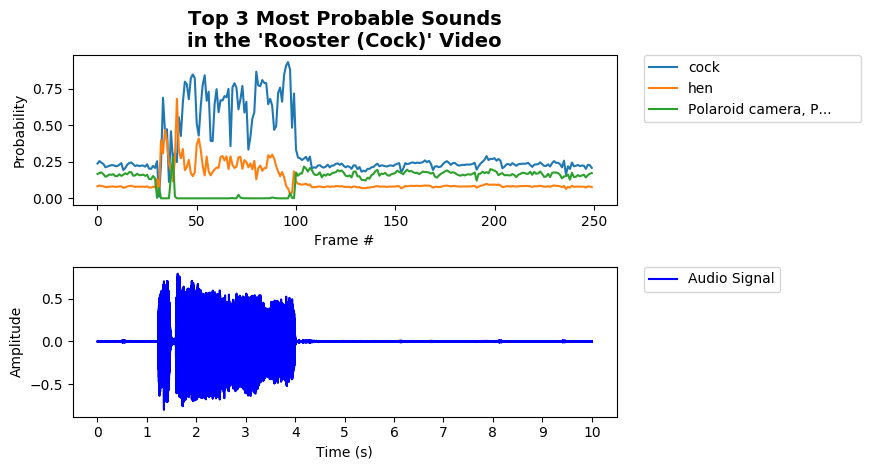
\includegraphics[width=\textwidth]{inf_rooster.png}}
   {\caption{\footnotesize The top graph shows the top three most probable sounds that AudioNet is able to classify from the rooster (cock) video for each frame.
             The bottom graph shows the raw audio signal from this video over the same time period.}
     \label{fig:inf_rooster}}
\end{figure}

\begin{figure}[h]
   \centerline{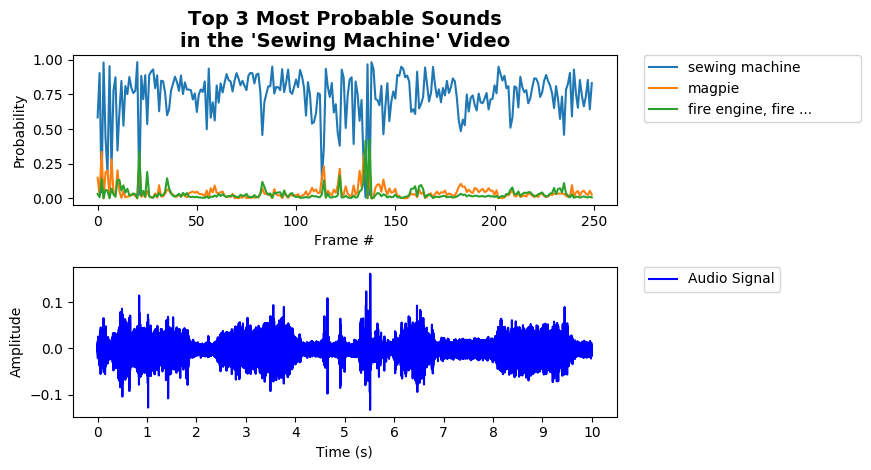
\includegraphics[width=\textwidth]{inf_sewing_machine.png}}
   {\caption{\footnotesize The top graph shows the top three most probable sounds that AudioNet is able to classify from the sewing machine video for each frame.
             The bottom graph shows the raw audio signal from this video over the same time period.}
     \label{fig:inf_sewing_machine}}
\end{figure}

\begin{figure}[h]
   \centerline{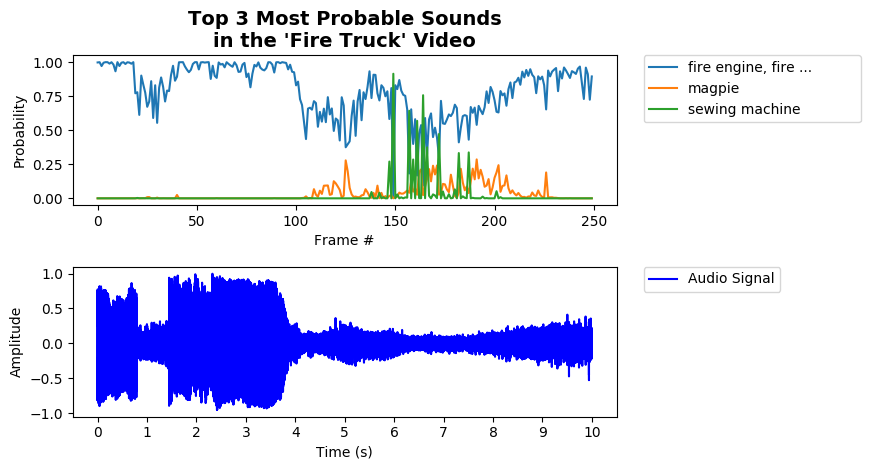
\includegraphics[width=\textwidth]{inf_fire_truck.png}}
   {\caption{\footnotesize The top graph shows the top three most probable sounds that AudioNet is able to classify from the fire truck video for each frame.
             The bottom graph shows the raw audio signal from this video over the same time period.}
     \label{fig:inf_fire_truck}}
\end{figure}

\begin{figure}[h]
   \centerline{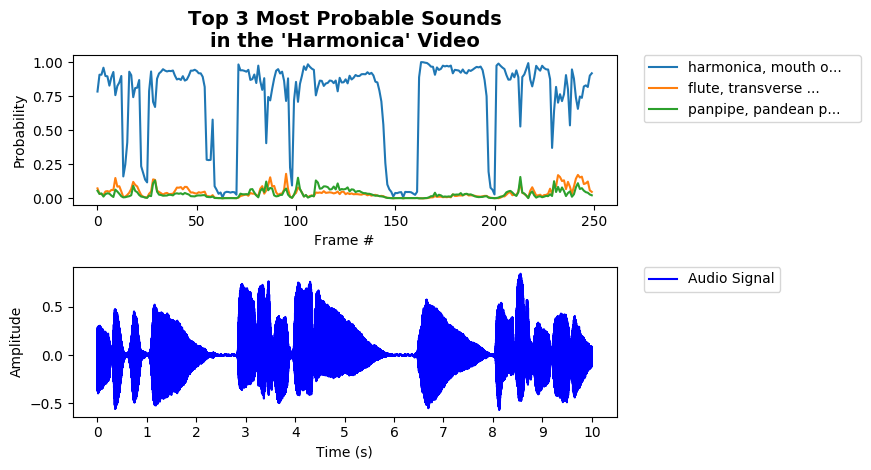
\includegraphics[width=\textwidth]{inf_harmonica.png}}
   {\caption{\footnotesize The top graph shows the top three most probable sounds that AudioNet is able to classify from the harmonica video for each frame.
             The bottom graph shows the raw audio signal from this video over the same time period.}
     \label{fig:inf_harmonica}}
\end{figure}

\begin{figure}[h]
   \centerline{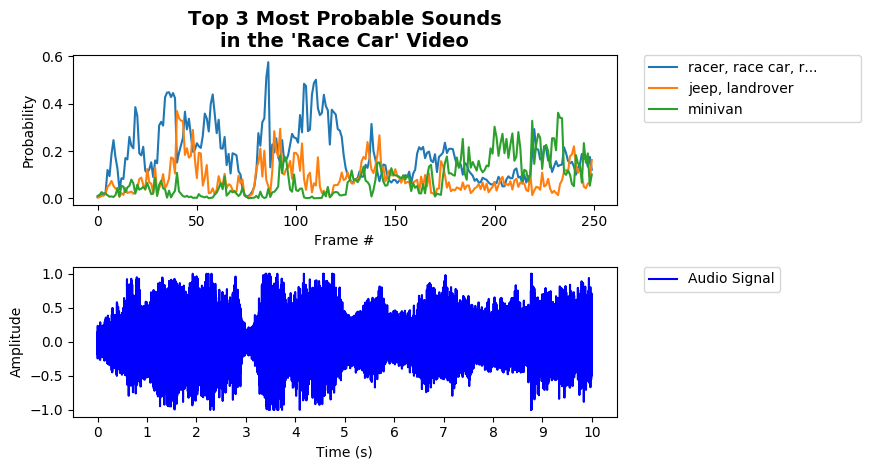
\includegraphics[width=\textwidth]{inf_race_car.png}}
   {\caption{\footnotesize The top graph shows the top three most probable sounds that AudioNet is able to classify from the race car video for each frame.
             The bottom graph shows the raw audio signal from this video over the same time period.}
     \label{fig:inf_race_car}}
\end{figure}

\begin{figure}[h]
   \centerline{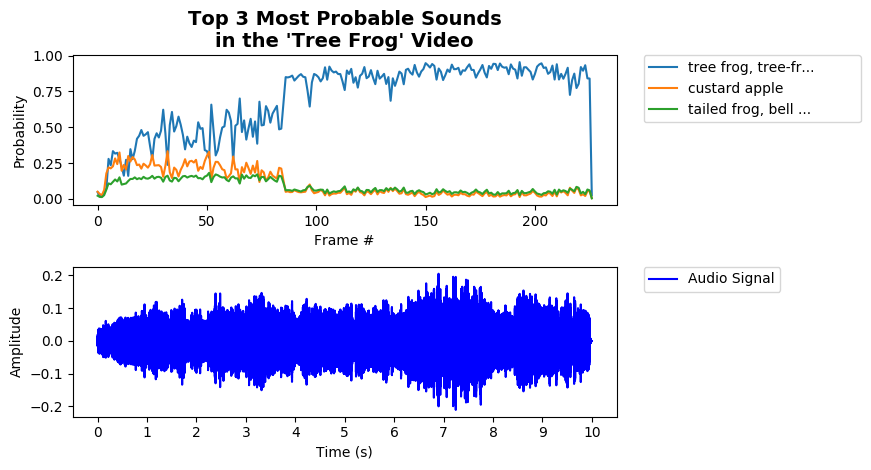
\includegraphics[width=\textwidth]{inf_tree_frog.png}}
   {\caption{\footnotesize The top graph shows the top three most probable sounds that AudioNet is able to classify from the tree frog video for each frame.
             The bottom graph shows the raw audio signal from this video over the same time period.}
     \label{fig:inf_tree_frog}}
\end{figure}

\begin{figure}[h]
   \centerline{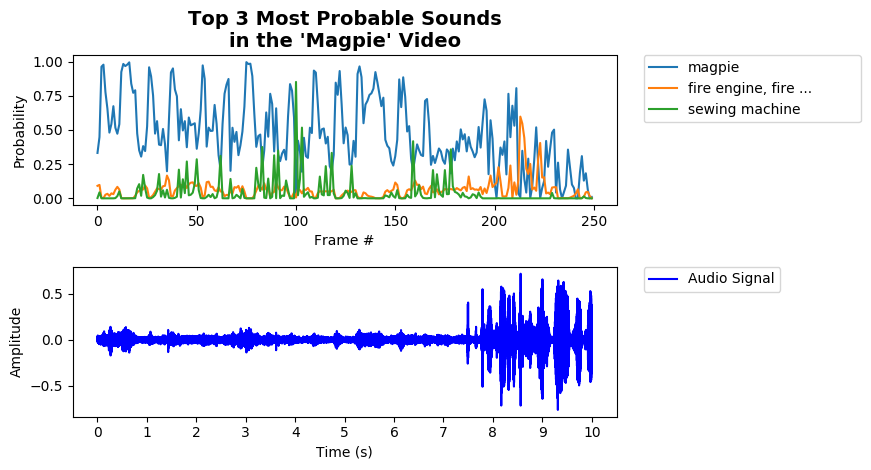
\includegraphics[width=\textwidth]{inf_magpie.png}}
   {\caption{\footnotesize The top graph shows the top three most probable sounds that AudioNet is able to classify from the magpie video for each frame.
             The bottom graph shows the raw audio signal from this video over the same time period.}
     \label{fig:inf_magpie}}
\end{figure}


%%%%%%%%%%%%%%%%%%%%%%%%%%%
%%  Appendix - Code
%%%%%%%%%%%%%%%%%%%%%%%%%%%
\section{AudioNet Python Modules}
\label{sec:pythonmodules}
This section contains the code of the core modules for AudioNet.
The code for the entire project can be found on GitHub at:

\noindent
\begin{center}
\url{https://github.com/AmyBryce/audionet}
\end{center}

\subsection{frames.py}
\label{subsec:frames.py}

{\setlength{\fboxsep}{10pt}
\scriptsize
\begin{Verbatim}[frame=leftline, numbers=left, xleftmargin=5mm]
import gzip
import pathlib
import shutil
import sys
import tempfile

import numpy as np

from moviepy.editor import VideoFileClip

def get(video_file, sample_period_msec = 40, audio_sample_rate = 16000):
    suffixes = pathlib.Path(video_file).suffixes
    if suffixes[-1] == '.gz':
        with tempfile.NamedTemporaryFile(mode="w+b", suffix=suffixes[-2]) as temp_file:
            with gzip.open(video_file) as video_contents:
                shutil.copyfileobj(video_contents, temp_file)
                temp_file.flush()
                clip = VideoFileClip(temp_file.name)
    else:
        clip = VideoFileClip(video_file)

    sample_period_sec = sample_period_msec / 1000.0
    if sample_period_sec > clip.duration:
        sample_period_sec = clip.duration

    subsampled_audio = clip.audio.set_fps(audio_sample_rate)

    samples_per_audio_frame = audio_sample_rate * sample_period_sec

    current_ts = 0
    video_frames = []
    audio_frames = []
    while current_ts + sample_period_sec <= clip.duration:
        video_frame = clip.get_frame(current_ts + sample_period_sec/2)
        video_frames.append(video_frame)

        audio_frame = subsampled_audio.subclip(
            current_ts,
            current_ts + sample_period_sec).iter_frames()
        audio_frame = np.array(list(audio_frame)).mean(1)
        audio_frame = audio_frame[:int(samples_per_audio_frame)]
        audio_frames.append(audio_frame)

        current_ts += sample_period_sec

    return {
        "video_frames" : video_frames,
        "audio_frames" : audio_frames
    }
\end{Verbatim}
}

\newpage
\subsection{train.py}
\label{subsec:train.py}

{\setlength{\fboxsep}{10pt}
\scriptsize
\begin{Verbatim}[frame=leftline, numbers=left, xleftmargin=5mm]
import frames
import gc
import json
import random
import sys
import time
import torch

import os.path

import audionet as an
import numpy as np
import torchvision.models.vgg as models
import torchvision.transforms as transforms

from PIL import Image

# Global, tunable parameters
num_epochs = 5000
video_sample_period_msec = 40
batch_size = 512
learning_rate = 1e-4

# Initialize an dictionary which will be used to dump per-epoch
# stats about the training after it is complete.
statistics = {
    "num_epochs": num_epochs,
    "video_sample_period_msec": video_sample_period_msec,
    "batch_size": batch_size,
    "learning_rate": learning_rate,
    "epochs": []
}

# Parse the arguments.
saved_model_path = None
for i, arg in enumerate(sys.argv):
    if arg == "-o":
        saved_model_path = sys.argv[i + 1]
        sys.argv.remove("-o")
        sys.argv.remove(saved_model_path)
        break

if not saved_model_path:
    print("You must supply an output path for"
          " the trained model with -o <path>",
          file=sys.stderr)
    sys.exit(1)

video_files = sys.argv[1:]

# Create a new audionet model.
# If GPUs are available, make sure to use them.
# Make sure it is possible to backpropagate the gradients through audionet.
audionet = an.Model()
if torch.cuda.is_available():
    audionet = torch.nn.DataParallel(audionet.cuda())
for param in audionet.parameters():
    param.requires_grad = True

# Load the pretrained vgg16 model.
# If GPUs are available, make sure to use them.
# Disallow backpropagation of the gradients through the pretrained vgg16 model.
vgg16 = models.vgg16(pretrained=True)
if torch.cuda.is_available():
    vgg16 = torch.nn.DataParallel(vgg16.cuda())
for param in vgg16.parameters():
    param.requires_grad = False

# Define some extra layers to pass the
# output through vgg16 and audionet.
softmax = torch.nn.Softmax()
logsoftmax = torch.nn.LogSoftmax()
kldivloss = torch.nn.KLDivLoss(reduce=False)

# Transforms to apply to each image frame for passing through vgg16.
# http://pytorch.org/docs/master/torchvision/models.html
image_transforms = transforms.Compose([
    transforms.ToTensor(),
    transforms.Normalize(
        mean=[0.485, 0.456, 0.406],
        std=[0.229, 0.224, 0.225])])

# Use a standard SGD optimizer to update the weigths in audionet.
optimizer = torch.optim.SGD(
    audionet.parameters(),
    lr=learning_rate,
    nesterov=True,
    momentum=0.9)

# Format the video and audio frames for processing.
paired_frames = []
for i, video_file in enumerate(video_files):
    print("Load Video {} of {}:".format(i + 1, len(video_files)))
    print("  Name: {}".format(video_file))

    frame_data = frames.get(
        video_file,
        video_sample_period_msec)

    file_names = [os.path.basename(video_file)] * len(frame_data["video_frames"])

    images = []
    for video_frame in frame_data["video_frames"]:
        img = Image.fromarray(video_frame, mode="RGB")
        img = img.resize((224, 224), resample=Image.NEAREST)
        img = image_transforms(img)
        images.append(img)

    paired_frames.extend(zip(file_names, images, frame_data["audio_frames"]))

# Start processing the video and audio frames.
for i in range(num_epochs):
    print("Epoch {} of {}:".format(i + 1, num_epochs))

    # Shuffle the paired frames so they are processed in a different order
    # than they were originally added in. This adds variance to the types of
    # sound processed each time we walk through the loop below.
    random.shuffle(paired_frames)

    # Add a dictionary to help collect statistics
    # about the training of this epoch.
    statistics["epochs"].append({})

    beg_time = time.time()
    for j in range(0, len(paired_frames), batch_size):
        # Pull the frame batches out of paired_frames.
        file_names = [pair[0] for pair in paired_frames[j:j+batch_size]]
        video_frames = [pair[1] for pair in paired_frames[j:j+batch_size]]
        audio_frames = [pair[2] for pair in paired_frames[j:j+batch_size]]

        # Use the optimizer to zero out all of the gradients in audionet.
        optimizer.zero_grad()

        # Format the video frame and audio frame batches for passing through
        # the vgg16 and audionet neural networks. Make sure and use GPUs if
        # they are available.
        image_tensor = torch.from_numpy(np.stack(video_frames)).float()
        audio_tensor = torch.from_numpy(np.stack(audio_frames)).float()
        if torch.cuda.is_available():
            image_tensor = image_tensor.cuda()
            audio_tensor = audio_tensor.cuda()
        image_input = torch.autograd.Variable(image_tensor)
        audio_input = torch.autograd.Variable(audio_tensor)

        # Pass the video frame batch through vgg16.
        vgg_output = vgg16(image_input)
        vgg_probs = softmax(vgg_output)

        # Pass audio frame batch through audionet.
        audionet_output = audionet(audio_input)
        audionet_log_probs = logsoftmax(audionet_output)

        # Compute the loss function as the KL
        # divergence between vgg16 and audionet.
        kldiv_output = kldivloss(audionet_log_probs, vgg_probs)
        kldiv_output = kldiv_output.sum(dim=1)

        # Sum the KL divergence across the entire batch.
        kldiv_average = kldiv_output.sum(dim=0)

        # Backpropogate the gradients through audionet.
        kldiv_average.backward()

        # Trigger the optimizer to update the weights
        # on all the layers in audionet.
        optimizer.step()

        # Gather stats about the kl-divergence computed for each video frame.
        for k in range(len(file_names)):
            statistics["epochs"][i].setdefault("videos", {})
            statistics["epochs"][i]["videos"].setdefault(file_names[k], {})
            statistics["epochs"][i]["videos"][file_names[k]].setdefault("kldiv_per_frame", [])
            statistics["epochs"][i]["videos"][file_names[k]]["kldiv_per_frame"].append(float(kldiv_output[k]))

        # Explicitly invoke the garbage collector
        # to cleanup any dangling references.
        gc.collect()

    end_time = time.time()

    training_time = end_time - beg_time
    statistics["epochs"][i]["training_time"] = training_time
    print("  Training Time: {:0.3f} s".format(training_time))

# Dump trained model into a file.
model_dir = os.path.join("output", "models")
model_path = os.path.join(model_dir, saved_model_path)
os.makedirs(model_dir, exist_ok=True)
if torch.cuda.is_available():
    audionet.module.save(model_path)
else:
    audionet.save(model_path)
print("Model written to: {}".format(model_path))

# Dump training statistics into a file.
stats_dir = os.path.join("output", "stats", "training")
stats_path = os.path.join(stats_dir, os.path.basename(saved_model_path) + ".stats.json")
os.makedirs(stats_dir , exist_ok=True)
with open(stats_path, 'w') as jsonfile:
    json.dump(statistics, jsonfile)
print("Model Statistics written to: {}".format(stats_path))
\end{Verbatim}
}

\newpage
\subsection{audionet.py}
\label{subsec:audionet.py}

{\setlength{\fboxsep}{10pt}
\scriptsize
\begin{Verbatim}[frame=leftline, numbers=left, xleftmargin=5mm]
import torch

class Model(torch.nn.Module):
    def __init__(self):
        super(Model, self).__init__()

        self.conv = torch.nn.Conv1d(
            in_channels=1,     # This is fixed to 1 for raw audio input.
            out_channels=16,
            kernel_size=64,
            stride=2,
            padding=32)

        self.maxpool = torch.nn.MaxPool1d(
            kernel_size=8,
            stride=1,
            padding=4)

        self.dense = torch.nn.Linear(
            in_features=16,    # This must match 'out_channels' from self.conv.
            out_features=1000) # This is fixed by imagenet.

    def forward(self, x):
        x = x.unsqueeze(1) # Add a channel dimension.
        x = self.conv(x)
        x = self.maxpool(x)
        x = torch.nn.functional.avg_pool1d(x, kernel_size=x.size()[2])
        x = x.squeeze(2) # Remove the averaged value's dimension.
        x = self.dense(x)
        return x

    def save(self, path):
        torch.save(self.state_dict(), path)


def loadModel(path):
    load = torch.load(path, map_location=(lambda storage, location: storage))
    model = Model()
    model.load_state_dict(load)
    return model
\end{Verbatim}
}

\newpage
\subsection{infer.py}
\label{subsec:infer.py}

{\setlength{\fboxsep}{10pt}
\scriptsize
\begin{Verbatim}[frame=leftline, numbers=left, xleftmargin=5mm]
import frames
import json
import os
import torch
import sys

import audionet as an

video_path = sys.argv[1]
model_path = sys.argv[2]
sample_period_msec = float(sys.argv[3])

frame_data = frames.get(video_path, sample_period_msec)

audionet = an.loadModel(model_path)
softmax = torch.nn.Softmax()

statistics = {
    "video_file": os.path.basename(video_path),
    "model_file": os.path.basename(model_path),
    "sample_period_msec": sample_period_msec,
    "frame_probabilities": []
}

for audio_frame in frame_data["audio_frames"]:
    audio_tensor = torch.FloatTensor(audio_frame).unsqueeze(0)
    audio_input = torch.autograd.Variable(audio_tensor)
    audionet_output = audionet(audio_input)
    audionet_probs = softmax(audionet_output)

    float_probs = [float(p) for p in audionet_probs.data.squeeze(0)]
    statistics["frame_probabilities"].append(float_probs)

# Dump the inference statistics to a file.
stats_dir = os.path.join("output", "stats", "inference", os.path.basename(model_path))
stats_path = os.path.join(
    stats_dir,
    os.path.basename(video_path) + "-{}.stats.json".format(int(sample_period_msec))
)
os.makedirs(stats_dir , exist_ok=True)
with open(stats_path, 'w') as jsonfile:
    json.dump(statistics, jsonfile)
print("Inference Statistics written to: {}".format(stats_path))
\end{Verbatim}
}


%%%%%%%%%%%%%%%%%%%%%%%%%%%%%%%%%%%%%%
% hier werden - zum Ende des Textes - die bibliographischen Referenzen
% eingebunden
%
% Insbesondere stehen die eigentlichen Informationen in der Datei
% ``bib.bib''
%
\newpage
\addcontentsline{toc}{section}{References}% Add to the TOC
\bibliographystyle{plain}
\bibliography{bib}

\end{document}
